% Keep this lesson within the framework's two-page limit while leaving room
% for the reaction-rate bookkeeping developed during class.
\tcbset{handout base/.append style={before skip=3pt,after skip=3pt}}

\HandoutSetup
  {NE 630}
  {05}
  {Using Cross-Section Data}
  {Read FNRP Sections 2.3--2.4. Identify the three reactor-neutron energy ranges and distinguish potential scattering from compound-nucleus reactions before class.}

\begin{document}
\MakeHandoutTitle

\begin{handoutcolumns}

\begin{fixedbox}{Macro objective}
For a neutron of energy $E$, determine the interactions it can undergo and
compute the probability that it undergoes a particular reaction.
\end{fixedbox}

\TermStrip{thermal, epithermal, and fast neutron; evaluated data; elastic and inelastic scattering; capture; absorption; fission; total cross section; potential scattering; compound nucleus; resonance; reaction-rate density; conditional probability}

\HandoutSection{1}{What do neutrons do?}

\begin{fixedbox}{Interaction bookkeeping}
Any interaction removes a neutron from its \emph{uncollided beam}; only some
interactions remove the incident neutron from the system.  For mutually
exclusive reaction channels $x$,
\[
 \sigma_t^i(E)=\sum_x\sigma_x^i(E),
 \qquad
 \Sigma_x^i(E)=n_i\sigma_x^i(E).
\]
Useful grouped cross sections include
\[
 \sigma_s\approx\sigma_e+\sigma_{in}+\cdots,
 \qquad
 \sigma_a=\sigma_\gamma+\sigma_f+\sigma_\alpha+\cdots.
\]
\end{fixedbox}

\begin{fixedbox}{Common neutron cross sections}
\scriptsize
\begin{tabularx}{\linewidth}{@{}l X@{}}
\toprule
$\sigma_x$ & reaction or interaction channel \\
\midrule
$\sigma_n$ or $\sigma_e$ & elastic scattering \\
$\sigma_{n'}$ or $\sigma_{in}$ & inelastic scattering \\
$\sigma_{2n}$ & $(n,2n)$ and related multiplicative reactions \\
\midrule
$\sigma_\gamma$ & radiative capture, $(n,\gamma)$ \\
$\sigma_f$ & fission \\
$\sigma_\alpha$ & $(n,\alpha)$ \\
$\sigma_a$ & absorption: $\sigma_\gamma+\sigma_f+\sigma_\alpha+\cdots$ \\
\midrule
$\sigma_t$ & total: sum over all exclusive channels \\
\bottomrule
\end{tabularx}
\normalsize
\end{fixedbox}

\begin{checkpoint}[Beam loss versus system loss]
Elastic scattering removes a neutron from the original beam: \RevealBlank[0.48in]{yes}.
It destroys that neutron: \RevealBlank[0.48in]{no}.  Which listed reactions can
increase the neutron population?
\RuledLines{1}
\end{checkpoint}

\switchcolumn

\HandoutSection{2}{Neutrons span many energies}

\begin{fixedbox}{Reactor-neutron energy ranges}
\scriptsize
\begin{tabularx}{\linewidth}{@{}>{\bfseries}l X X@{}}
\toprule
range & interval & physical landmark \\
\midrule
thermal & $10^{-3}\unit{eV}\le E<1\unit{eV}$ & target thermal motion matters \\
epithermal & $1\unit{eV}\le E<0.1\unit{MeV}$ & many resolved and unresolved resonances \\
fast & $0.1\unit{MeV}\le E\le10\unit{MeV}$ & fission-birth-energy range \\
\bottomrule
\end{tabularx}
\smallskip
The useful range spans about ten orders of magnitude. At room temperature,
$kT\approx0.0253\unit{eV}$; fission neutrons are born with mean energy about
$2\unit{MeV}$.
\normalsize
\end{fixedbox}

\begin{fixedbox}{Examples of normalized neutron spectra}
\centering
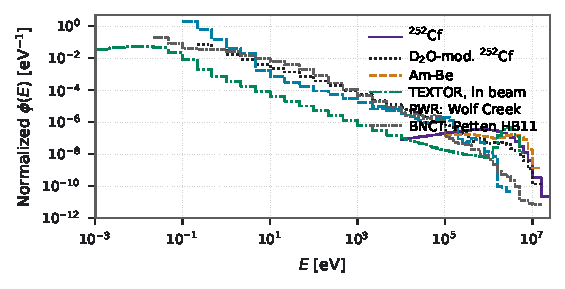
\includegraphics[width=\linewidth]{spectra.pdf}
\end{fixedbox}

\begin{checkpoint}[Do not confuse the two functions]
A spectrum $\phi(E)$ describes \RevealBlank[1.25in]{neutrons available} at
energy $E$; a cross section $\sigma_x^i(E)$ describes
\RevealBlank[1.45in]{interaction propensity} for nuclide $i$ and channel $x$.
\end{checkpoint}

\HandoutSection{3}{From evaluated data to a rate}

\begin{boardbox}{Use one consistent neutron energy}
For nuclide $i$ and reaction $x$, follow
\[
 \boxed{\sigma_x^i(E)}
 \;\xrightarrow{\ \times n_i\ }\;
 \boxed{\Sigma_x^i(E)}
 \;\xrightarrow{\ \times\phi\ }\;
 \boxed{R_x^i(E)}.
\]
\[
 [\sigma]=\unit{cm^2},\quad [\Sigma]=\unit{cm^{-1}},\quad
 [R]=\unit{reactions\,cm^{-3}\,s^{-1}}.
\]
Before summing, verify that every $\sigma_x^i$ is evaluated at the same $E$
and that the reaction categories do not overlap.
\end{boardbox}

\end{handoutcolumns}

\newpage
\begin{handoutcolumns}

\HandoutSection{4}{The balancing act}

\begin{fixedbox}{Decompose the total reaction-rate density}
For a monoenergetic flux $\phi$,
\[
\begin{aligned}
 R_t
 &=\Sigma_t\phi
  =\left(\sum_i\Sigma_t^i\right)\phi
  =\left(\sum_i n_i\sigma_t^i\right)\phi \\
 &=\left(\sum_i n_i\sum_x\sigma_x^i\right)\phi
  =\sum_i\sum_x R_x^i.
\end{aligned}
\]
The useful partial sums are
\[
 R_x=\sum_iR_x^i,
 \qquad
 R_t^i=\sum_xR_x^i,
 \qquad
 R_t=\sum_xR_x=\sum_iR_t^i.
\]
\end{fixedbox}

\begin{boardbox}{Read each rate ratio as a conditional probability}
\footnotesize
\begin{align*}
 \frac{R_x}{R_t}
   &: \text{reaction is }x\text{, given an interaction},\\[2pt]
 \frac{R_t^i}{R_t}
   &: \text{target is }i\text{, given an interaction},\\[2pt]
 \frac{R_x^i}{R_t^i}
   &: \text{reaction is }\RevealBlank[0.36in]{$x$}\text{, given target }i,\\[2pt]
 \frac{R_x^i}{R_x}
   &: \text{target is }\RevealBlank[0.36in]{$i$}\text{, given reaction }x,\\[2pt]
 \frac{R_f}{R_a}
   &: \text{an absorption produces }\RevealBlank[0.58in]{fission}.
\end{align*}
The common flux cancels from these ratios. For a homogeneous mixture at a
fixed $E$,
\[
 \boxed{P(x\mid\text{interaction})
 =\frac{\sum_i n_i\sigma_x^i}{\sum_i n_i\sigma_t^i}}.
\]
\normalsize
\end{boardbox}

\begin{fixedbox}{Fission-neutron production}
\[
 \dot n_{\mathrm{birth}}=\sum_i\bar\nu^iR_f^i,
 \qquad
 \bar\nu_{\mathrm{mix}}
 =\frac{\sum_i\bar\nu^iR_f^i}{R_f}.
\]
The first expression is a neutron-production-rate density; the second is the
rate-weighted mean neutrons born per fission.
\end{fixedbox}

\begin{checkpoint}[Conditional is not absolute]
Over a uniform path of length $L$, combine Lesson 4 with the rate ratio:
\[
 P(\text{first interaction is }x\text{ by }L)
 =\MathBlank[1.75in]{\frac{\Sigma_x}{\Sigma_t}
   \left(1-e^{-\Sigma_tL}\right)}.
\]
\end{checkpoint}

\switchcolumn

\HandoutSection{5}{Apply the bookkeeping}

\begin{fixedbox}{A one-to-one $\mathrm{H_2O}$--${}^{235}\mathrm{U}$ mixture}
At the selected neutron energy, take one water molecule per ${}^{235}$U atom.
Thus $n_{\mathrm H}:n_{\mathrm O}:n_{\mathrm U}=2:1:1$; write the three as
$2n_0$, $n_0$, and $n_0$. Unlisted cross sections are zero in this exercise.

\smallskip
\centering\scriptsize
\begin{tabular}{@{}lccc@{}}
\toprule
nuclide & $\sigma_e$ & $\sigma_\gamma$ & $\sigma_f$ \\
\midrule
H-1 & $20\unit{b}$ & $0.1\unit{b}$ & --- \\
O-16 & $4\unit{b}$ & --- & --- \\
${}^{235}$U & $15\unit{b}$ & $100\unit{b}$ & $500\unit{b}$ \\
\bottomrule
\end{tabular}
\normalsize
\end{fixedbox}

\begin{boardbox}{Build the competing rate strengths}
Because every term contains $n_0\phi_0$, compare the effective microscopic
strengths:
\footnotesize
\begin{align*}
 \frac{R_e}{n_0\phi_0}
   &=2(20)+1(4)+1(15)=\MathBlank[0.56in]{59}\unit{b},\\
 \frac{R_a}{n_0\phi_0}
   &=2(0.1)+1(100+500)=\MathBlank[0.66in]{600.2}\unit{b},\\
 \frac{R_t}{n_0\phi_0}
   &=\MathBlank[0.54in]{59}+\MathBlank[0.66in]{600.2}
     =\MathBlank[0.66in]{659.2}\unit{b}.
\end{align*}
\normalsize
\end{boardbox}

\begin{checkpoint}[If a neutron interacts, what happens?]
\footnotesize
\begin{align*}
 P(e\mid\mathrm{int})
   &=\frac{59}{659.2}=\MathBlank[0.60in]{0.0895}\approx\RevealBlank[0.44in]{0.09},\\
 P(\mathrm{H\ elastic}\mid\mathrm{int})
   &=\frac{2(20)}{659.2}=\MathBlank[0.60in]{0.0607}\approx\RevealBlank[0.44in]{0.06},\\
 P(\mathrm{U\ absorption}\mid\mathrm{int})
   &=\frac{100+500}{659.2}=\MathBlank[0.60in]{0.910}\approx\RevealBlank[0.44in]{0.91},\\
 P(f\mid\mathrm{absorbed})
   &=\frac{500}{600.2}=\MathBlank[0.60in]{0.833}\approx\RevealBlank[0.44in]{0.83}.
\end{align*}
\normalsize
\end{checkpoint}

\begin{takeawaybox}[The reusable recipe]
At a fixed energy: read $\sigma_x^i(E)$, weight by each
\RevealBlank[1.08in]{number density $n_i$}, form reaction rates, then normalize
the desired partial rate by the rate named in the condition.
\end{takeawaybox}

\end{handoutcolumns}
\end{document}
